\documentclass[11pt,a4paper]{article}
\usepackage[T1]{fontenc}
\usepackage[margin=23mm]{geometry}
\usepackage{amsmath,amssymb,bm,graphicx,booktabs,hyperref}
\setlength{\parindent}{0pt}
\setlength{\parskip}{4pt}
\setlength{\emergencystretch}{2em}
\title{Contour Geometry and Local Differential Factors\\in Excitation-Current Coordinate Reduction}
\author{Winding Factor Research Study}
\date{25 October 2026}
\begin{document}
\maketitle
\begin{abstract}
This follow-up separates the numerical geometry of the conventional contour estimator from local differential compensation directions. It reuses canonical measurements and saved 80-neighbour derivative estimates. One contour level and adjacent excitation pair provide an initial comparison of intersection means, arclength centroids and robust location statistics. Local scalar and two-axis factors are visualized independently by nominal excitation group. The reference calculation and previously fitted coordinate models are unchanged. No global flux model or new parameter optimization is introduced.
\end{abstract}

\section{Reference and questions}
The existing study considers $\bm\psi=(\psi_d,\psi_q)^\mathsf T$ as a function of $(i_d,i_q,i_e)$. The conventional reduction uses $s=i_d+k i_e$, while its estimator averages the measured-current coordinates of retained mesh-edge crossings at selected d-flux levels $\lambda$:
\begin{equation}
\bar{\bm i}_g(\lambda)=\frac{1}{N_g}\sum_{r=1}^{N_g}\bm i_{g,r}(\lambda),\qquad
k_A=\operatorname{mean}_{g,\lambda}\frac{|\bar i_{d,g+1}-\bar i_{d,g}|}{\bar i_{e,g+1}-\bar i_{e,g}}.
\end{equation}
The reference uses exactly 100 equally spaced levels in the middle 25--75\% of the pooled d-flux value range and retains only finite, numerically nonzero ratios. Nominal excitation defines groups; measured excitation enters the coordinates and denominators. Display-only extended levels do not enter $k_A$.

The questions are whether intersection density and available contour geometry influence this statistic, how local differential factors vary over the observed domain, and what separates them from a globally useful coordinate transformation. Approximate q-sign symmetry is a hypothesis to inspect, not a constraint to impose.

\section{Contour representatives and available support}
The arithmetic edge mean is not an arclength centroid. For retained piecewise-linear contour segments with endpoints $\bm a_j,\bm b_j$, physical stator-current length $\ell_j=\|(b_{d,j}-a_{d,j},b_{q,j}-a_{q,j})\|$ gives the exact segment-integral centroid
\begin{equation}
\bm c_L=\frac{\sum_j\ell_j(\bm a_j+\bm b_j)/2}{\sum_j\ell_j}.
\end{equation}
The excitation coordinate is linearly interpolated along each segment. Isolated retained crossings enter the reference mean but carry no segment length. Componentwise median and 10\%-per-tail trimmed means are compared on both the actual crossings and equal-arclength samples. These statistics depend on their sampling measure and are not automatically geometric representatives.

Equal-arclength and equal-per-segment sampling keep the interpolant fixed. A deterministic half-density, hull-preserving remesh changes the interpolated field as well as the intersection distribution; its change cannot be attributed exclusively to weighting. Open endpoints identify available mesh boundaries or edge-filter effects, not physical contour termination. Mirror queries use the full original scattered interpolant: their finite-query fraction describes convex-hull support rather than complete edge-filtered contour support.

For any representative $(c_d,c_q)$, the diagnostic
\begin{equation}
\epsilon_g=\widetilde\psi_{d,g}(c_d,c_q)-\lambda
\end{equation}
measures departure from the intended contour level. It is not a reconstruction RMSE. Even a length centroid need not lie on a nonlinear contour. A fixed-$i_q$ comparison separately keeps all detected roots and forms a factor only if each group has exactly one root; branch ambiguity is not resolved by arbitrary pairing.

\begin{figure}[htbp]\centering
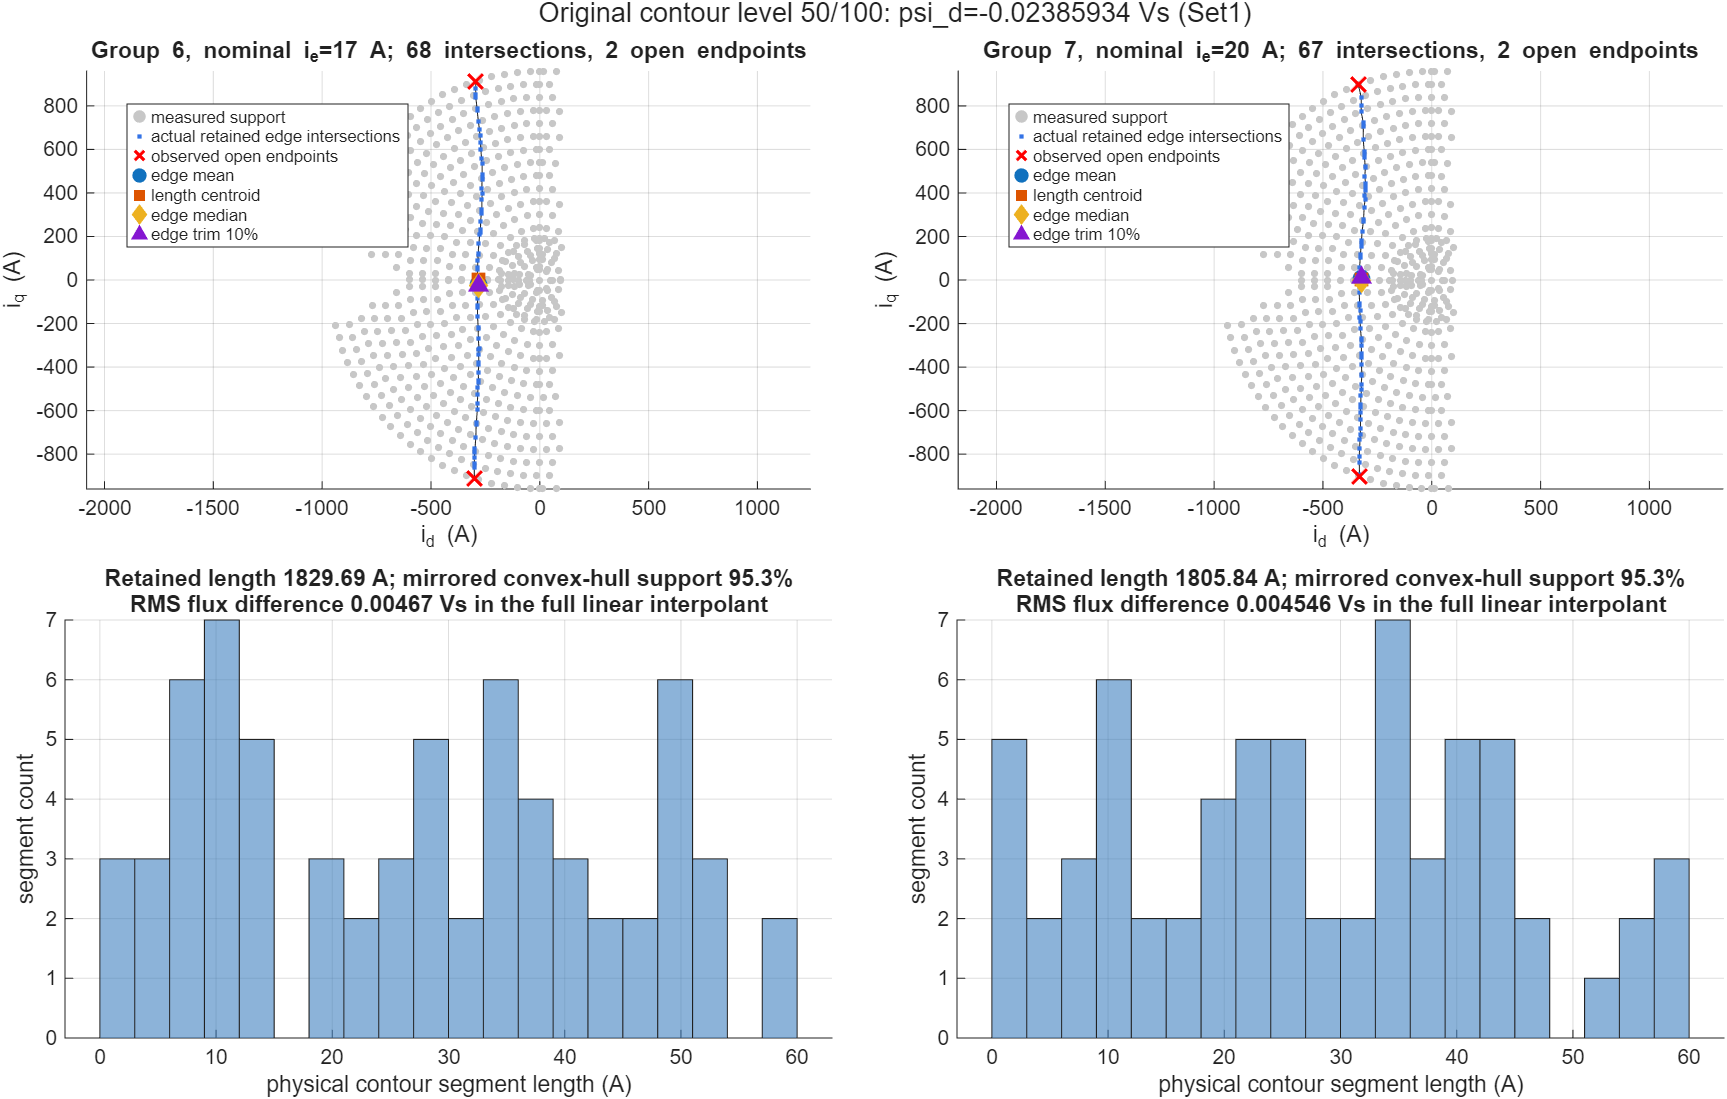
\includegraphics[width=\linewidth]{../figures/contour_averaging_set1_g6_7_level50_1.png}
\caption{First diagnostic: Set 1, nominal 17/20 A, original contour level 50. The contours, retained intersections, available endpoints and four representatives are shown together. The lower panels describe physical segment lengths and mirrored interpolant support. This single example does not establish a global estimator ranking.}
\end{figure}

\subsection{First observed comparison}
At $\lambda=-0.0238593398$ Vs, the reference mean is reproduced exactly. Its pair factor is 13.0010684 A/A, compared with 13.3751163 A/A for length centroids, a 2.877\% change. The two q-coordinate means change from $(-22.846,7.989)$ A to $(1.376,0.393)$ A. Both length centroids still depart from the selected level. Each contour has two observed open endpoints on the mesh hull. Mirrored interpolant support is approximately 95.33\%; mirrored flux RMS differences are approximately 4.67 and 4.55 mVs, so exact symmetry is not observed. These observations do not identify a unique physical cause or show that length weighting predicts flux more accurately.

\section{Local scalar and two-axis compensation}
Using $L_{xy}=\partial\psi_x/\partial i_y$, define
\begin{equation}
\bm a=\begin{bmatrix}L_{dd}\\L_{qd}\end{bmatrix},\quad
\bm b=\begin{bmatrix}L_{de}\\L_{qe}\end{bmatrix},\qquad
k_{\rm loc}=\frac{\bm a^\mathsf T\bm b}{\bm a^\mathsf T\bm a}.
\end{equation}
This is the local differential least-squares optimum for $\|\bm b-k\bm a\|^2$ with equal component weights. It is not a global flux-error optimum. The existing scalar mask requires valid local affine derivatives and $\|\bm a\|>0.1\operatorname{median}\|\bm a\|$.

The two-axis factors instead solve
\begin{equation}
J\begin{bmatrix}k_d\\k_q\end{bmatrix}=\bm b,\qquad
J=\begin{bmatrix}L_{dd}&L_{dq}\\L_{qd}&L_{qq}\end{bmatrix}.
\end{equation}
Finite saved derivatives and $\operatorname{rcond}(J)\ge10^{-3}$ define the numerical screen. Thresholds $10^{-4}$ and $10^{-2}$ are reported as a sensitivity comparison. This is not a calibrated measurement-uncertainty bound, and $L_{dq}=L_{qd}$ is not imposed. All 24,590 saved points pass these screens; minimum per-set reciprocal condition estimates are approximately 0.170, 0.169 and 0.210.

\begin{table}[htbp]\centering\small
\caption{Observed local-factor 5th--95th percentiles (A/A), using saved derivatives. Percentiles describe spatial variation of estimates, not confidence intervals.}
\begin{tabular}{lrrr}\toprule
Set & $k_{\rm loc}$ & $k_d$ & $k_q$\\\midrule
1 & 4.27--15.43 & 4.25--15.57 & -4.32--3.88\\
2 & 4.37--15.48 & 4.30--15.61 & -4.05--4.04\\
3 & 4.19--16.27 & 3.67--16.21 & -7.08--4.76\\\bottomrule
\end{tabular}
\end{table}
The previously optimized global Method F constants are reused, not refitted: $(14.3367,-0.0256)$, $(14.1870,-0.0918)$ and $(14.6271,-0.7879)$ A/A. Their fitting criterion differs from pointwise derivative cancellation. Spatial factor variation does not by itself measure reconstruction error.

\begin{figure}[htbp]\centering
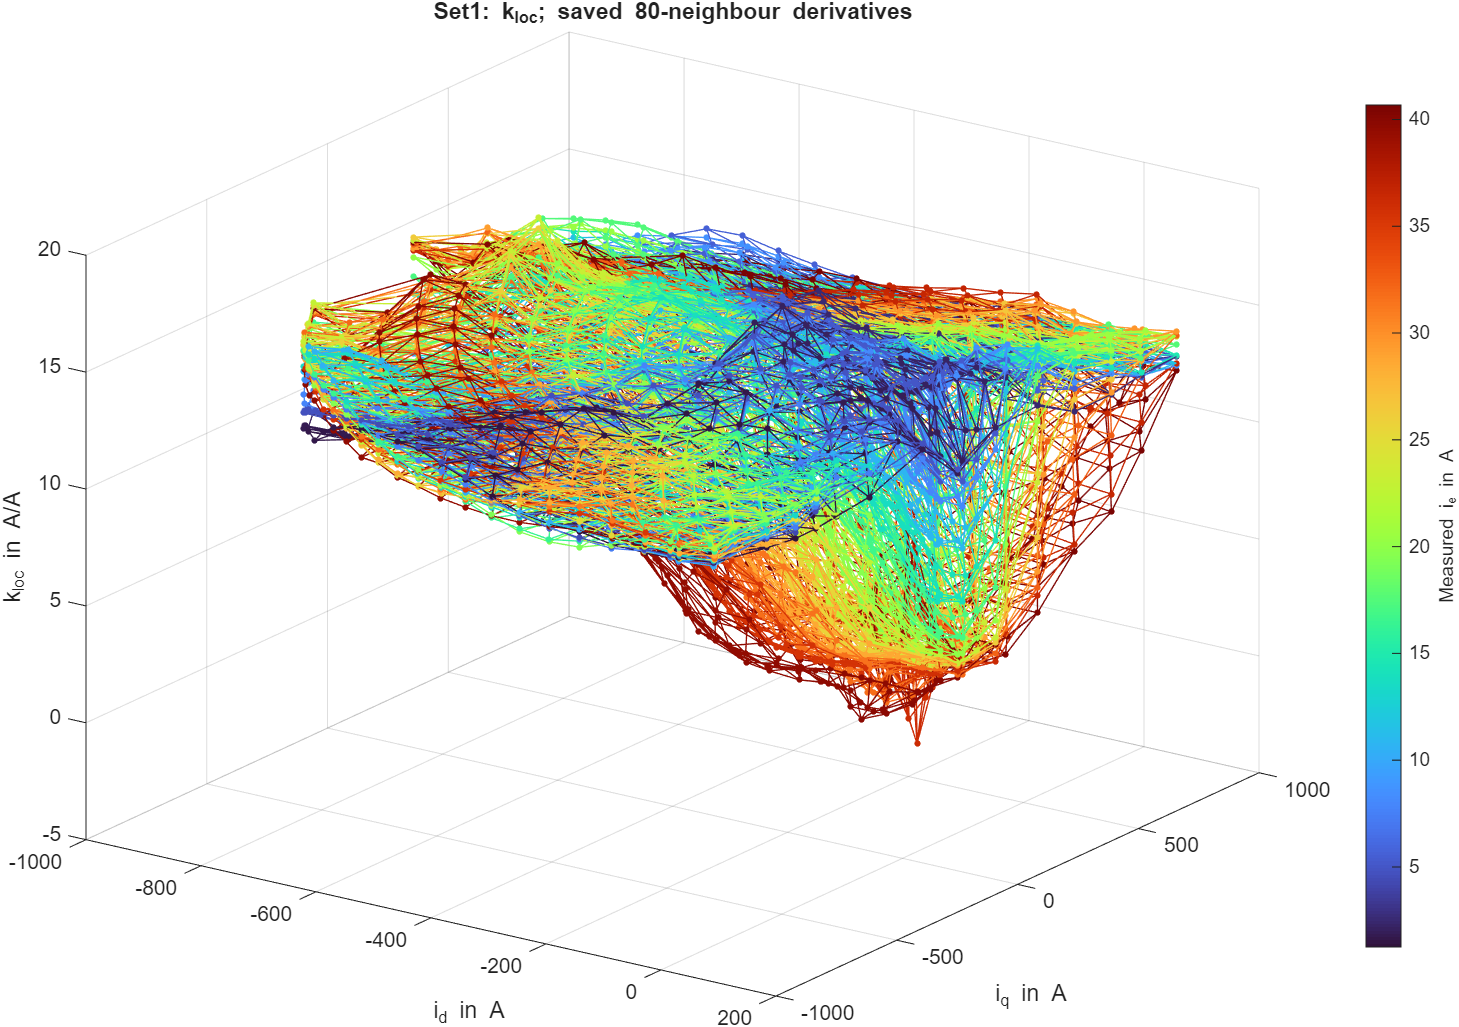
\includegraphics[width=0.92\linewidth]{../figures/local_kloc_set1.png}
\caption{Set 1 local differential least-squares factors over physical stator currents. Each nominal excitation group has its own original-point mesh and measured-excitation colour. Invalid vertices are removed without retriangulating holes; groups are not connected. Interactive checkboxes control each mesh and its points together.}
\end{figure}

\section{What remains open}
A common two-axis shift $(i_d+k_d i_e,i_q+k_q i_e)$ is different from using one d-axis shift for $\psi_d$ and another for $\psi_q$. The latter construction generally has different reduced coordinates for its two outputs. The former is the existing Method F when the factors are constants.

For smooth spatially varying factors, a local compensation direction is
\begin{equation}
V=\partial_{i_e}-k_d(\bm i)\partial_{i_d}-k_q(\bm i)\partial_{i_q}.
\end{equation}
If $J\bm k=\bm b$ holds, $V\bm\psi=0$. Reduced coordinates would have to be first integrals, $Vs_d=Vs_q=0$; simply substituting local factors into $i_d+k_d(\bm i)i_e$ and $i_q+k_q(\bm i)i_e$ adds derivatives of the coefficient fields. Smooth nonvanishing one-dimensional directions have local flow coordinates, but global continuation, support and single-valuedness require additional analysis.

Further work should extend the same contour diagnostics over levels and groups, distinguish density effects from changes to the interpolant, and investigate incomplete support, small denominators and sensitivity to derivative neighbourhoods. The existing determinant/nonparallelism diagnostics, global weighting differences and integrated-versus-differential shifts remain relevant. Methods D, E and G are prior work, not newly optimized candidates here. No claim of improved flux accuracy follows from these first diagnostics, and no new global flux-fit study is included.
\end{document}
